\chapter{OMNeT++}
\label{cha:omnet}

OMNeT++ represents a open source simulation framework written in C++.
It provides a object oriented modular discrete event network simulation framework.
The commercial supported version is OMNEST and provides licensing models, whereas OMNeT++ is only available for academic or non-profit use.
The intention of OMNeT++ is providing infrastructure for writing simulations for various fields; especially the field of network simulations.
For this thesis the current newest version of OMNeT++ 4.6 was used and analyzed.

Simulations developed with OMNeT++ are based on different components, which provide functionality for communication and topologies.

\section{Components}
\label{sec:omnet_components}
Within an OMNeT++ simulation different components are used to represent the simulated system.
Each component is described with a \emph{network description} (NED) file and can be enhanced with C++ code.
The \emph{NED} file contains information about the component, which is necessary for connecting and designing the simulated system, such as gates, submodules and parameters.

The different types of components and their sense is explained in the next sections.

\subsection{Network}
\label{sec:omnet_components_network}
The outermost component is a network, which consists of other components like modules and channels.
The simulated topology and the connections between modules are defined within the network.
All instantiated modules, optional parameters and the connections in between the modules are defined in the networks \emph{NED} file. \cite[section 3.2.1]{omnet_manual}

\subsection{Modules}
\label{sec:omnet_components_modules}
Modules represent functional groups of different complexities.
There are two types of modules available in OMNeT++.

A simple module is the smallest part within a simulated OMNeT++ hierarchy and represent a functional unit.
For this functional unit the behavior for handling messages, the possible connections and additional parameters can be defined. \cite[section 3.3]{omnet_manual}
The possible connections of modules are represented by gates, which can be connected to a channel or directly to other gates.

Multiple simple modules can be connected via channels and condensed to a compound module.
Such compound modules can be used in the same way as simple modules, but represent bigger functional groups.
Compound modules define, in the same way as networks, the instantiated submodules and the connections in between them. \cite[section 3.4]{omnet_manual}
For OMNeT++ a network and a compound module is the same component just with different values for the built in property \emph{@isNetwork}.

An example network including simple modules connected to a compound module is shown in figure \ref{fig:OMNeTComponents}.
Each module shown in figure \ref{fig:OMNeTComponents} defines two gates which can ether be an input, output or bidirectional gate.

\begin{figure}
    \centering
    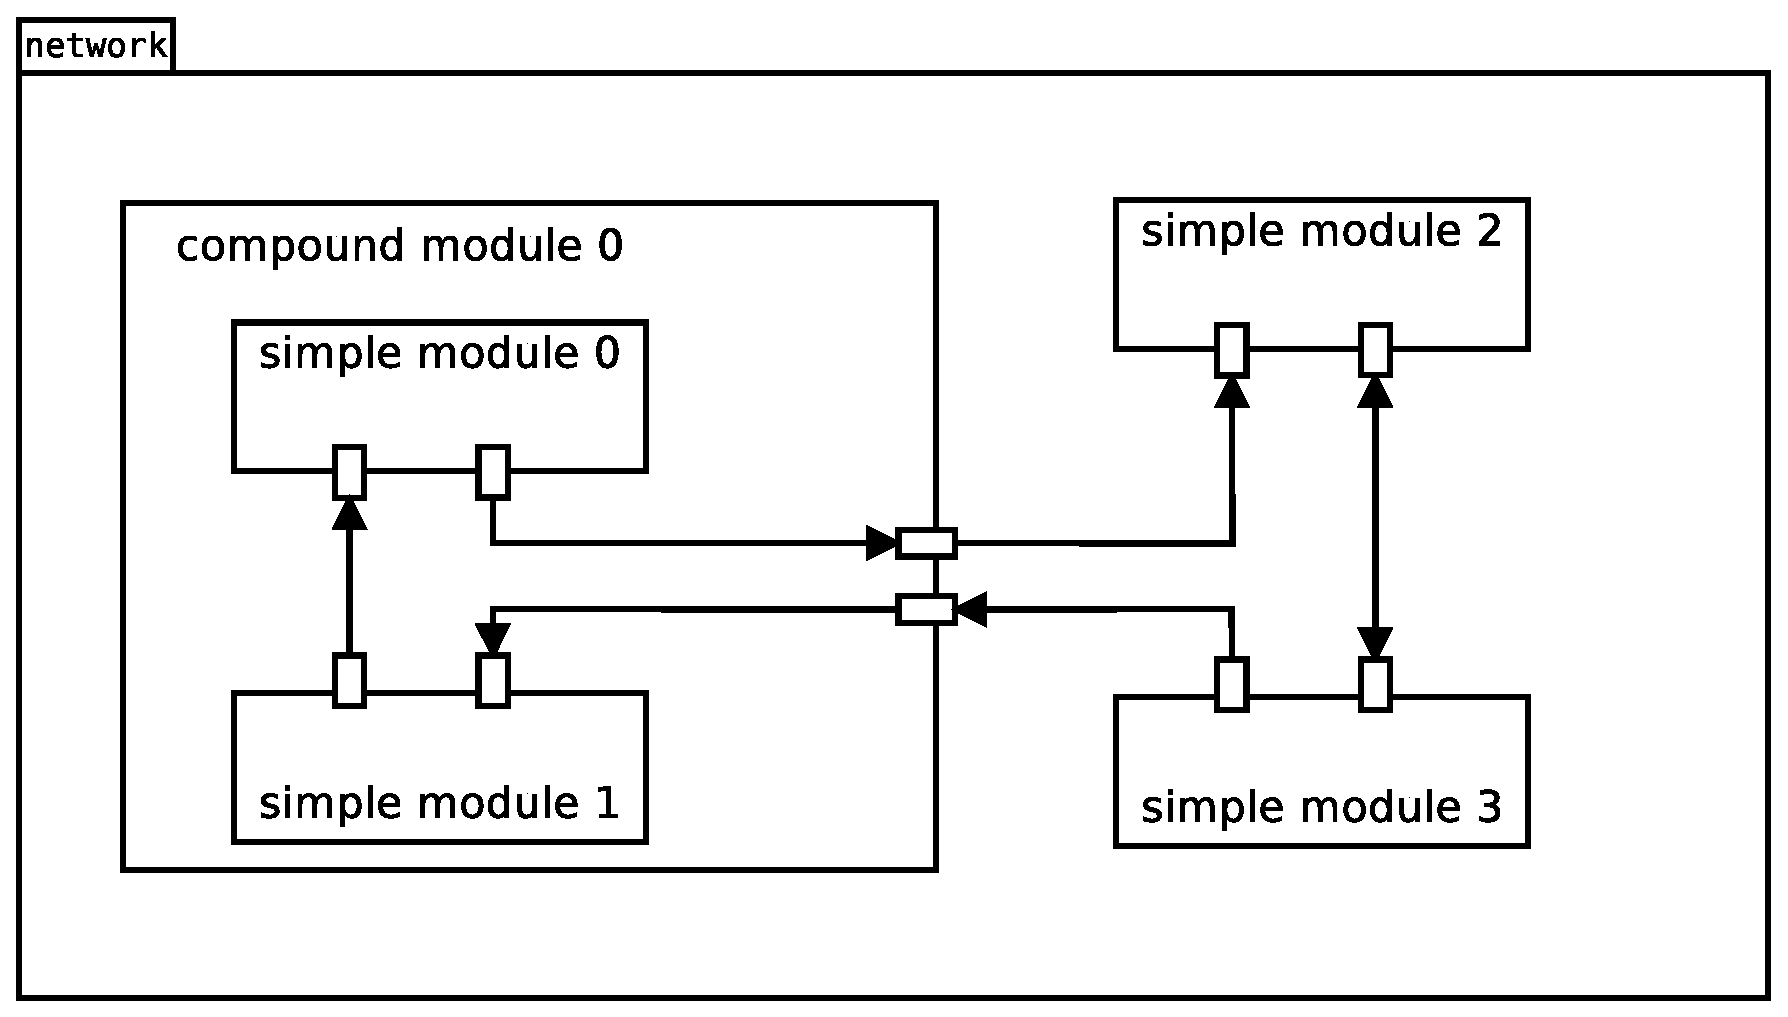
\includegraphics[width=0.9\columnwidth]{OMNeTComponents.eps}
    \caption{OMNeT++ components in an example network}
    \label{fig:OMNeTComponents}
\end{figure}

Specific functionality for custom components is implemented in the linked C++ code.
This assignment is usually done with identical names of the \emph{NED} file and the C++ code, but can also be done manually with the \emph{@class} property.
Examples and the combination of \emph{NED} files and C++ code is shown in \cite[chapter 3, chapter 4]{omnet_manual}.
The components can embed any functionality implemented in C/C++.
The usage of external libraries or language features is not limited, but must be used with care due to the effect on simulation performance.
OMNeT++ provides functionalities for accessing the simulation environment and for example reading the value of a defined \emph{NED} parameter or send a message via a gate.

The functionality of a compound module is given by the submodules and their connections.
A simple module is implemented by overriding specific methods following one of the two strategies:

\begin{itemize}
    \item Using the \emph{handleMessage} method a module can react to incoming messages.
    Using this strategy the module is only activated when a message is received.
    The methods \emph{send}, \emph{scheduleAt} and \emph{cancelEvent} can be used within \emph{handleMessage} for sending messages, scheduling self-messages and cancellation of scheduled self-messages. \cite[section 4.4.1]{omnet_manual}
    
    \item The second strategy uses the method \emph{activity} and is also called \emph{process style} strategy.
    The method \emph{activity} is called by the simulation runtime as coroutine and can be implemented in the same way as a normal thread or process on an operating system.
    Beside the available methods of the first strategy, additional methods can be used within \emph{activity}.
    Using the method \emph{receive} the module waits until a message is received.
    Waiting a specific amount of simulation time is achieved with the \emph{wait} method.
    A simple module using the \emph{activity} method is called as coroutine in the simulation library and are scheduled non-preemptively.
    I.e. the activity method is not interrupted by the simulation and has to suspend by itself.
    This is done by waiting for a received message or waiting a specific amount of time. \cite[section 4.4.2]{omnet_manual}
\end{itemize}

\subsection{Channels}
\label{sec:omnet_components_channels}
The connections in between modules can be realized in different ways.
An direct connection of two gates transports the transmitted messages immediately.
For applying transportation parameters (e.g. delay, latency, jitter) the connection can be established with a channel.
The OMNeT++ framework provides three built in channels for direct usage or sub classing.

\begin{itemize}
    \item The \emph{IdealChannel} represents the same behavior as a direct connection between gates and transmits each message immediately.
    \item The \emph{DelayChannel} provides a \emph{delay} parameter for configuring a constant delay for each message.
    Additionally there is the possibility to disable the channel and drop all containing messages.
    \item The \emph{DatarateChannel} provides the \emph{datarate} parameter for a variable data rate
\end{itemize}

Such a channel can implement a simple delayed transportation or complex customized functionality. \cite[section 3.5]{omnet_manual}

For implementing a custom Channel three Methods must be implemented:

\begin{description}
    \item[isTransmissionChannel] returns if the channel is a transmission channel, i.e. the transmission duration is calculated and set within the packet
    This type of channel only affects messages of type \emph{cPacket} or of derived types.
    \item[getTransmissionFinishTime] returns the finish time of the transmission for messages of type \emph{cPacket} or derived types.
    \item[processMessage] models the behavior of the channel and its functionality.
\end{description}

The general behavior of the channel is implemented in \emph{processMessage}.
In this method the results can be stored in a provided structure, which allows a dropping of the message and a change of the resulting transmission time. \cite[section 4.8]{omnet_manual}

\subsection{Parameters}
\label{sec:omnet_components_parameters}
Each component can define various parameters for configuration of their behavior.
The value of these parameters can be assigned in different ways.
The assignment from a \emph{NED} file can be done directly, via inheritance, or via a compound module or network which contains the component.
All parameters can also be set via a configuration file (e.g. omnetpp.ini) or interactively requested from the user.
For the case of no such assignment a parameter can also define a default value. \cite[section 3.6]{omnet_manual}


\subsection{Messages}
\label{sec:omnet_components_messages}
Transmitted data are encapsulated in another component called messages.
Messages are a fundamental component of a OMNeT++ simulation as they does not only transport data they can also represent functional messages like jobs, events or tasks.
The meaning behind a message is depending on the written simulation and the simulated system.

These messages can also be customized for holding a specific set of data like a protocol header, checksum, etc. or other specific data.
The existing message class \emph{cMessage} and its derived specialization \emph{cPacket} provide different members and methods which can be used for simulations.
These include control information, type information, time stamp, etc. and are included for making developing a simulation easier.
Adding a few simple datafields to a message can be ether done by subclassing \emph{cMessage} or \emph{cPacket} or using the \emph{NED} syntax in special \emph{.msg} files.
By defining a custom message using \emph{NED} a customized subclass will be generated by the simulation and can be normally used as Message. %TODO find reference

Any module can send a message via its gates by using the \emph{send} methods or send it to itself as \emph{self-message} with \emph{scheduleAt}.
The mechanism of messages is also used for implementing timeouts, timers, etc. by sending a specific message to the current module.
Therefore the method \emph{scheduleAt} takes a absolute simulation and a message as parameters and sends the given message at the given point to the current module.
These \emph{self-message} is handled by the same function as any other message coming from other modules.
For the identification of \emph{self-messages} there is a built in method \emph{isSelfMessage} available.
A scheduled \emph{self-message} can be canceled via the method \emph{cancelEvent} taking the scheduled message. \cite[section 4.7.1]{omnet_manual}

The \emph{send} methods takes the message to send and the used gate as parameter.
For defining the gate the defined name, the id or the object itself can be used. \cite[section 4.7.2]{omnet_manual}
When the transmission of the messages should occur at a later time, there is a built in functionality given with the \emph{sendDelayed} methods.
These methods work in the same way as the default \emph{send} methods but take an additional parameter which represents the delay. \cite[section 4.7.6]{omnet_manual}

Messages can also be sent directly to gates of defined modules without the need of a connection to the current module.
This is called \emph{direct sending} and can be useful when multiple sender modules send to a single input gate.
An example for this usage is shown in figure 
Such a gate should be declared with the \emph{@diretIn} property to avoid notifications about a not connected gate. \cite[section 4.7.5]{omnet_manual}

Additional handling of messages as broadcasts and retransmission requires attention to the owner of messages.
By sending a message its owner changes to the simulation core and furthermore to the received module.
Therefore for sending a message to multiple modules or resending a message the explicit copying of a message via \emph{dup} is necessary. \cite[section 4.7.3]{omnet_manual}

%TODO enhance
%More information about messages and the possibilities of customized messages are given in \cite[chapter 5]{omnet_manual}.

Each message sent ether by another module or by the current module itself represents an event for the simulation with an according time, at which this event should happen, or the message should be delivered/received.
The execution and the handling of such created events is done by the simulation core and defines the execution order and the performance of the simulation.
The different types of simulations and the simulation core of OMNeT++ is discussed in chapter \ref{cha:simulation}.
\section{Simulation results}
\label{sec:omnet_results}
\emph{OMNeT++} provides multiple functionalities for recording and saving different results of a simulation.


\subsection{Simulation library}
\label{sec:omnet_results_sim_lib}
The traditional way to record simulation results is using the simulation library functions to record vectors or scalars of different objects.

Since OMNeT++ 4.1 the newer strategies using \emph{signals} and \emph{statistics} are available and provide alternative methods for results recording.

\subsection{Signals}
\label{sec:omnet_results_signals}
Signals provide a functionality for a communication between modules which are not directly connected via their gates.
The usage of signals follows the \emph{publisher/subscriber} principle, i.e. modules can register callback objects to a specific signal.
If a new value for the signal is emitted all registered callback objects are notified.

Signals are defined in the \emph{NED} file of the according module or channel and can be accessed via the library call \emph{signal} and the defined name of the signal. %TODO check


\subsection{Statistics}
\label{sec:omnet_results_statistics}



\section{Running an OMNeT++ simulation}
\label{sec:omnet_running}
A OMNeT++ simulation is defined by a configuration file (\emph{.ini}-file).

\subsection{Configuration}
\label{sec:omnet_running_config}
This configuration file can be given by a command line parameter, by default the \emph{omnetpp.ini} file is used.
The configuration files includes every information and parameter regarding the simulation.

The simulated network must be defined, all other parameters are optional.



A simulation application developed with OMNeT++ can be run in different ways using different simulation environments.

\subsection{Tkenv}
\label{sec:omnet_running_tkenv}
OMNeT++ provides the graphical environment \emph{Tkenv} for developing simulations.
Various possibilities for graphical representation are useful for demographic purposes.
This environment is based on the opensource framework \emph{Eclipse} and provides the integrated development environment (\emph{IDE}) for OMNeT++ simulations.

\subsection{Cmdenv}
\label{sec:omnet_running_cmdenv}
The other environment for running \emph{OMNeT++} simulations is \emph{Cmdenv}, which represents a command line interface.
Using this environment no graphical user interface is shown, or will be updated.
This simulation method is recommended for batch simulations or running simulations with an increased runtime.